\section{Polar Form}

\subsection{Derivative of Polar Form}
\begin{equation}
    \frac{dy}{dx}=\frac{\frac{dr}{d\theta}\sin{(\theta)}+r\cos{(\theta)}}{\frac{dr}{d\theta}\cos{(\theta)}-r\sin{(\theta)}}
\end{equation}

\subsection{Switching to coordinates}
\begin{equation}
    r\sin{(\theta)}=y
\end{equation}
\begin{equation}
    r\cos{(\theta)}=x
\end{equation}

\subsection{Switching from coordinates}
\begin{equation}
    r=\sqrt{x^2+y^2}
\end{equation}
\begin{equation}
    \theta=\tan^{-1}{\left(\frac{y}{x}\right)}
\end{equation}

\subsection{Polar Equation That You Need To Remember}
\subsubsection{Lines}
    \begin{equation}
        r\cos{(\theta)}=a
    \end{equation}
    
    \begin{equation}
        r\sin{(\theta)}=b
    \end{equation}
    \begin{figure}[H]
        \centering
        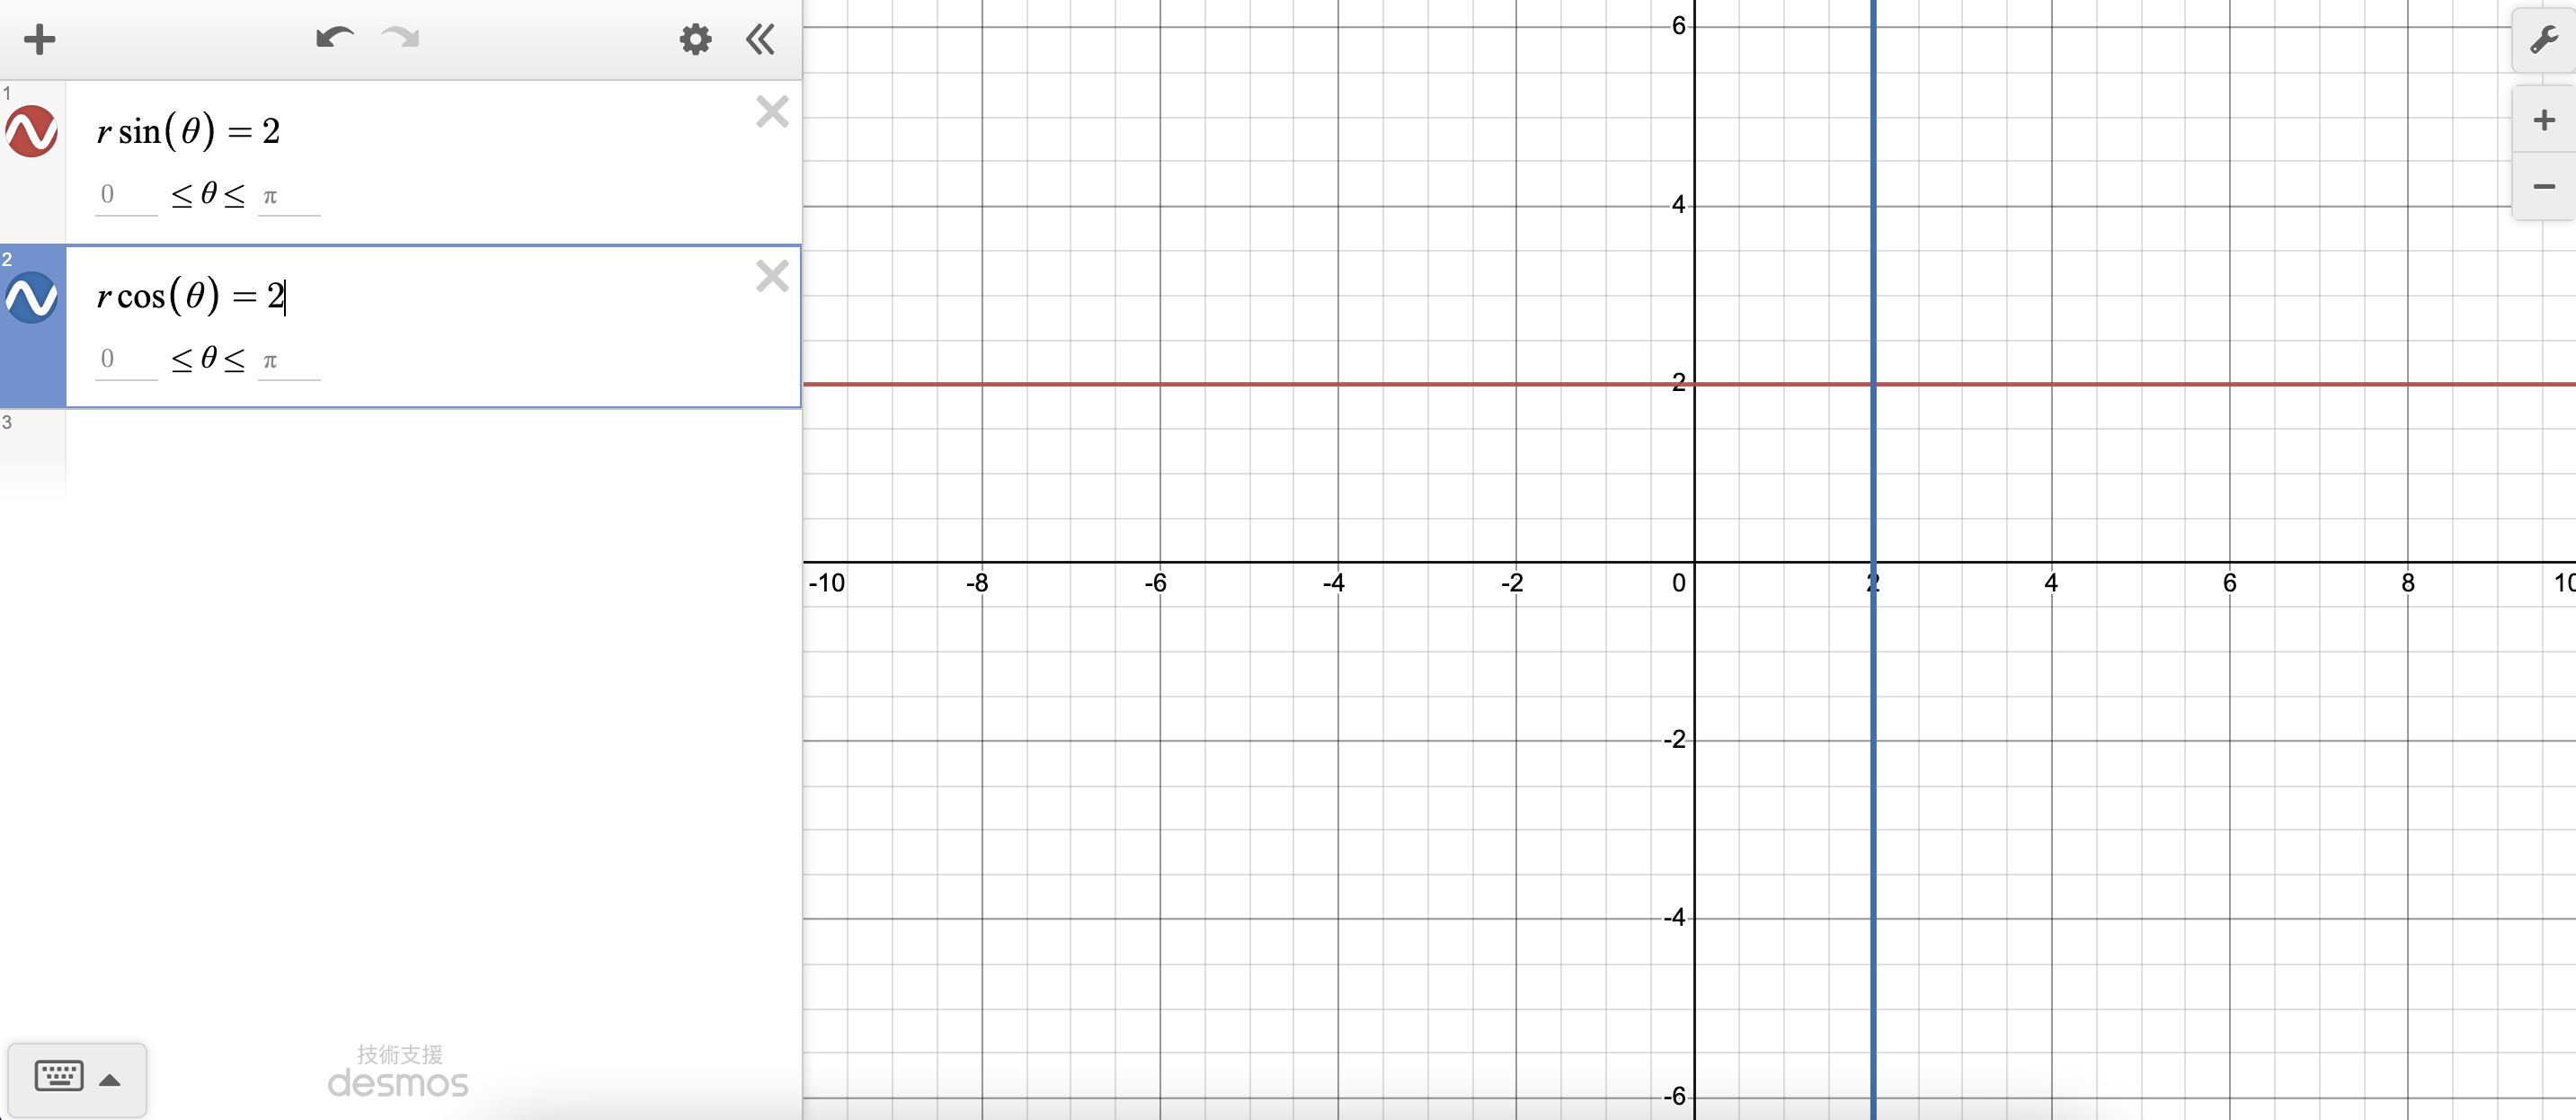
\includegraphics[width=\textwidth]{Pictures/Polar Line.png}
        \caption[]{Polar Lines \footnotemark}
        \label{polar lines}
    \end{figure}
    \footnotetext{Created using Desmos}
    \newpage
    
\subsubsection{Cardioid}
    \begin{equation}
        a-b\cos{(\theta)}
    \end{equation}
    There are 3 cases with cardioid: $a>b$, $a=b$ and $a<b$
    
    \begin{multicols}{3}
    \begin{figure}[H]
        \centering
        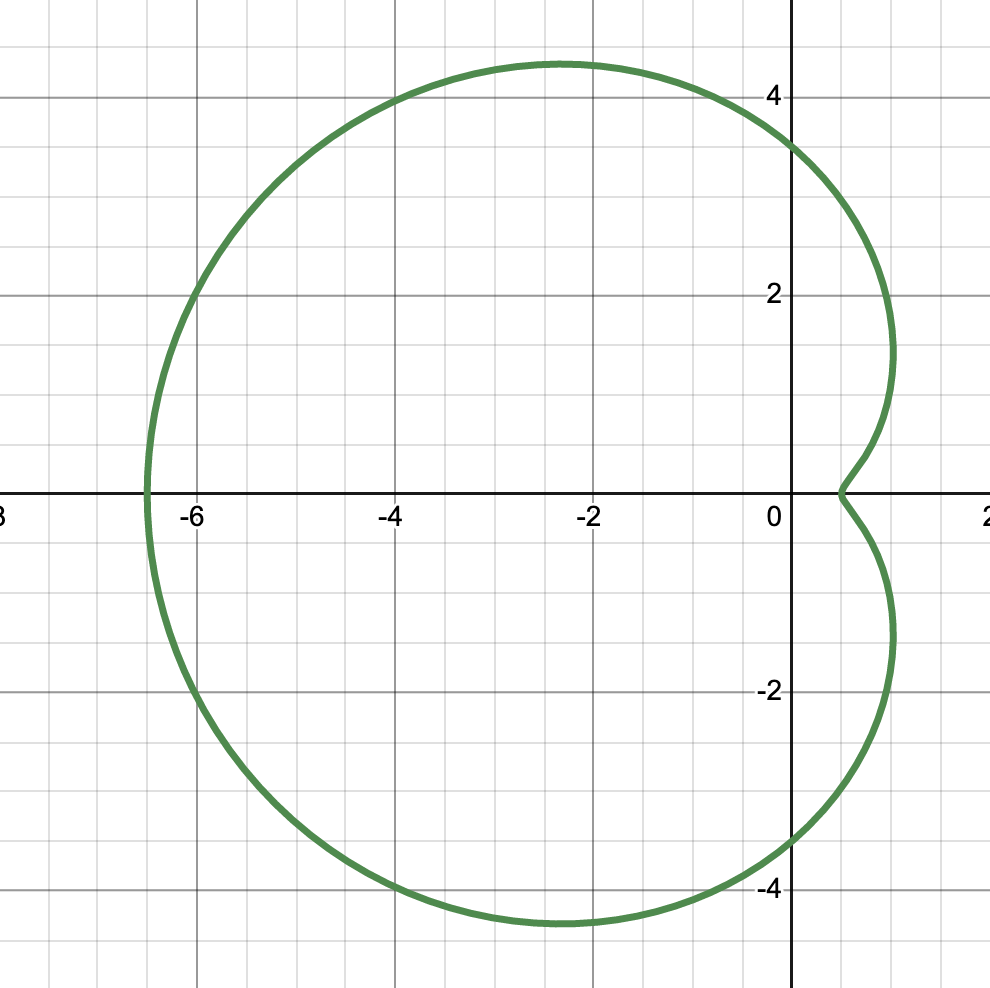
\includegraphics[width=5cm]{Pictures/Polar Form/Bigger.png}
        \caption[]{$a>b$ \footnotemark[2]}
        \label{a>b}
    \end{figure}
    \begin{figure}[H]
        \centering
        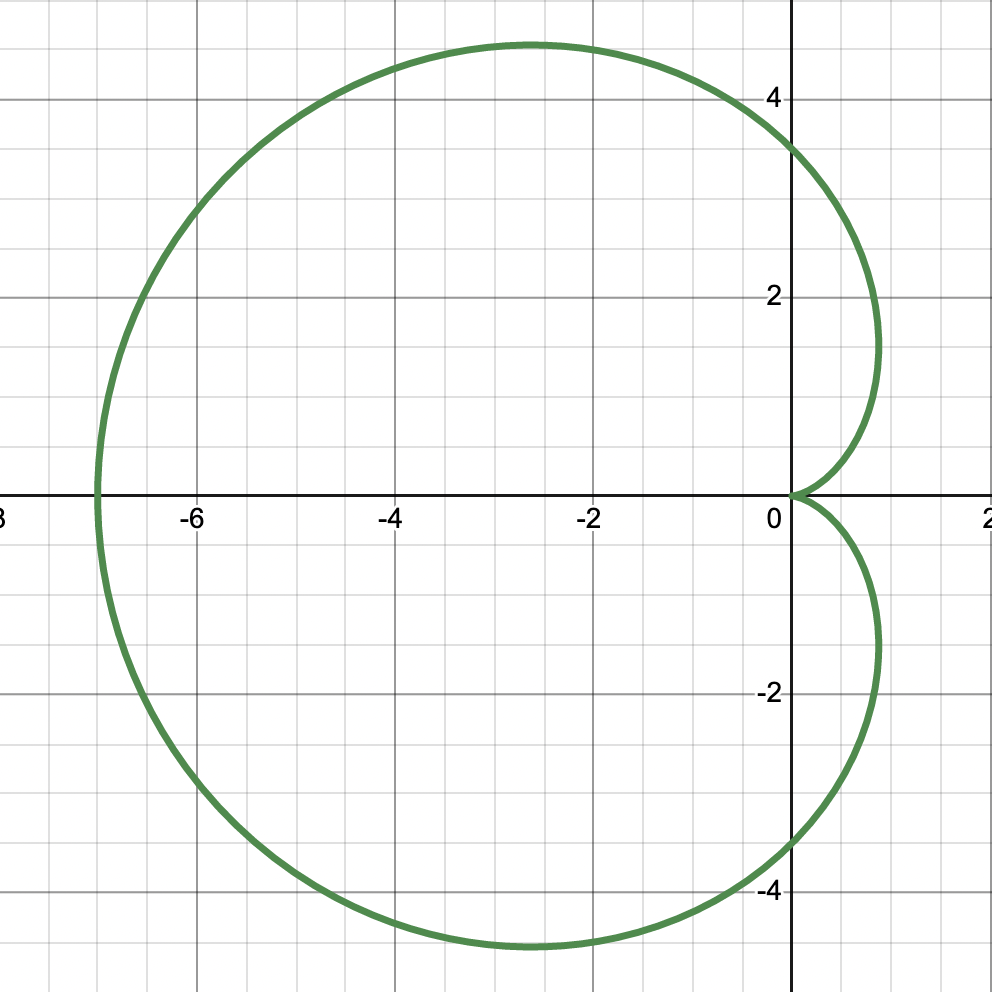
\includegraphics[width=5cm]{Pictures/Polar Form/Equal.png}
        \caption[]{$a=b$ \footnotemark[2]}
        \label{a=b}
    \end{figure}
    \begin{figure}[H]
        \centering
        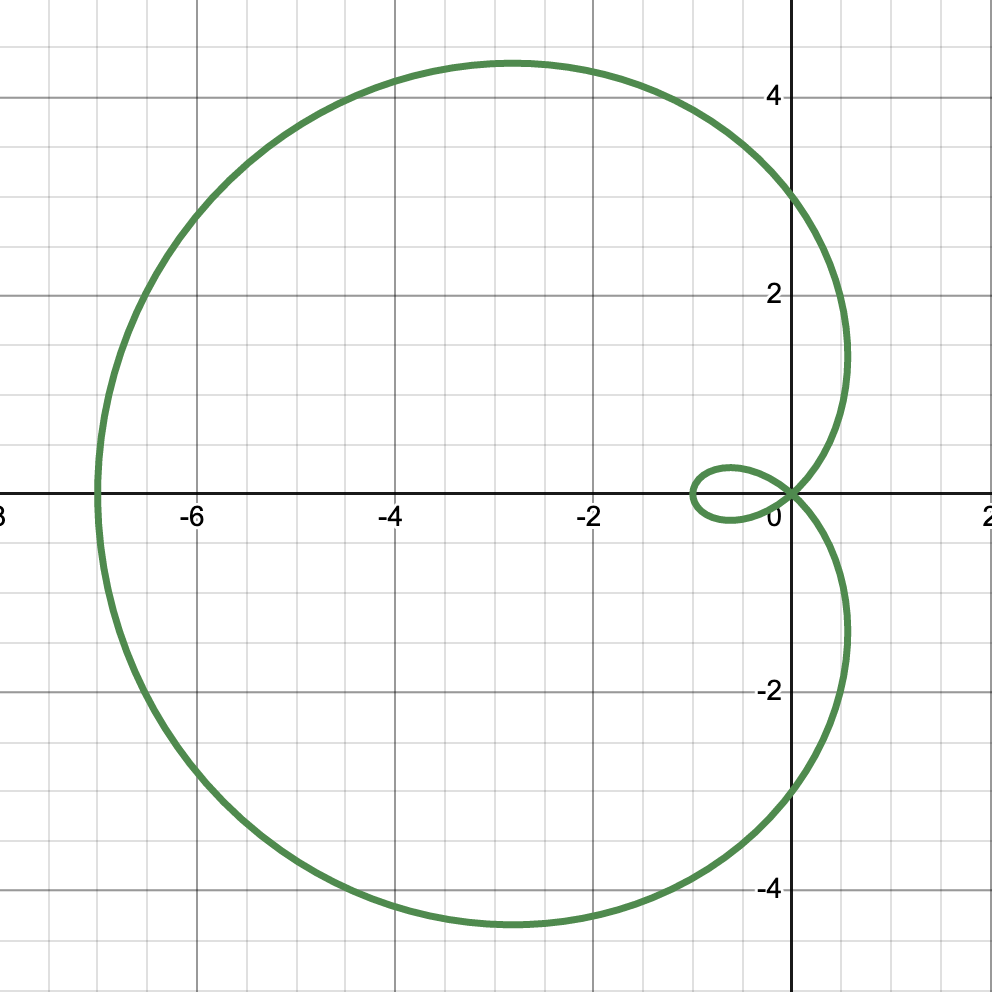
\includegraphics[width=5cm]{Pictures/Polar Form/Smaller.png}
        \caption[]{$a<b$ \footnotemark[2]}
        \label{a<b}
    \end{figure}
    \end{multicols}
    \footnotetext[2]{Created using Desmos}
    \begin{center}
        That's footnote, not exponent.
    \end{center}
    
    \noindent If it is a plus sign, simply flip everything
    \begin{equation}
        a+b\cos{(\theta)}
    \end{equation}
    \begin{multicols}{3}
    \begin{figure}[H]
        \centering
        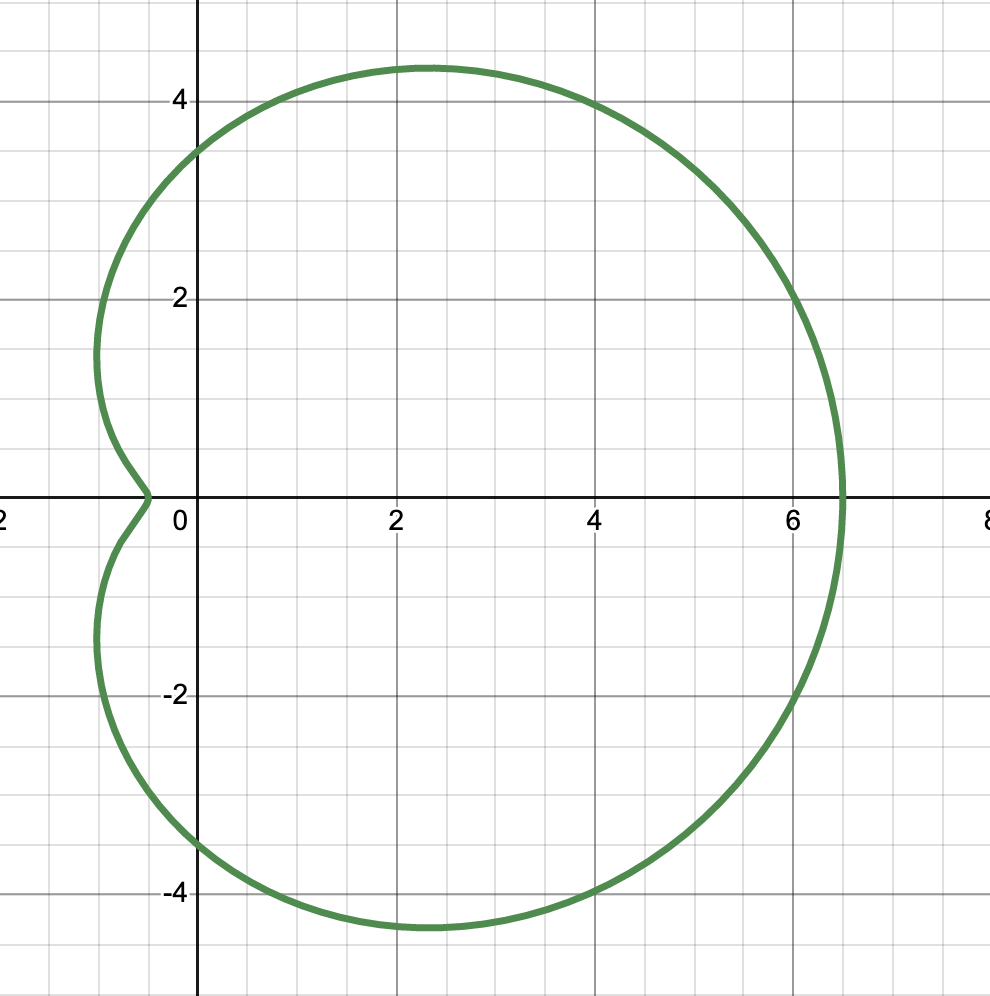
\includegraphics[width=5cm]{Pictures/Polar Form/BiggerReflect.png}
        \caption[]{$a>b$ \footnotemark[2]}
        \label{a>b}
    \end{figure}
    \begin{figure}[H]
        \centering
        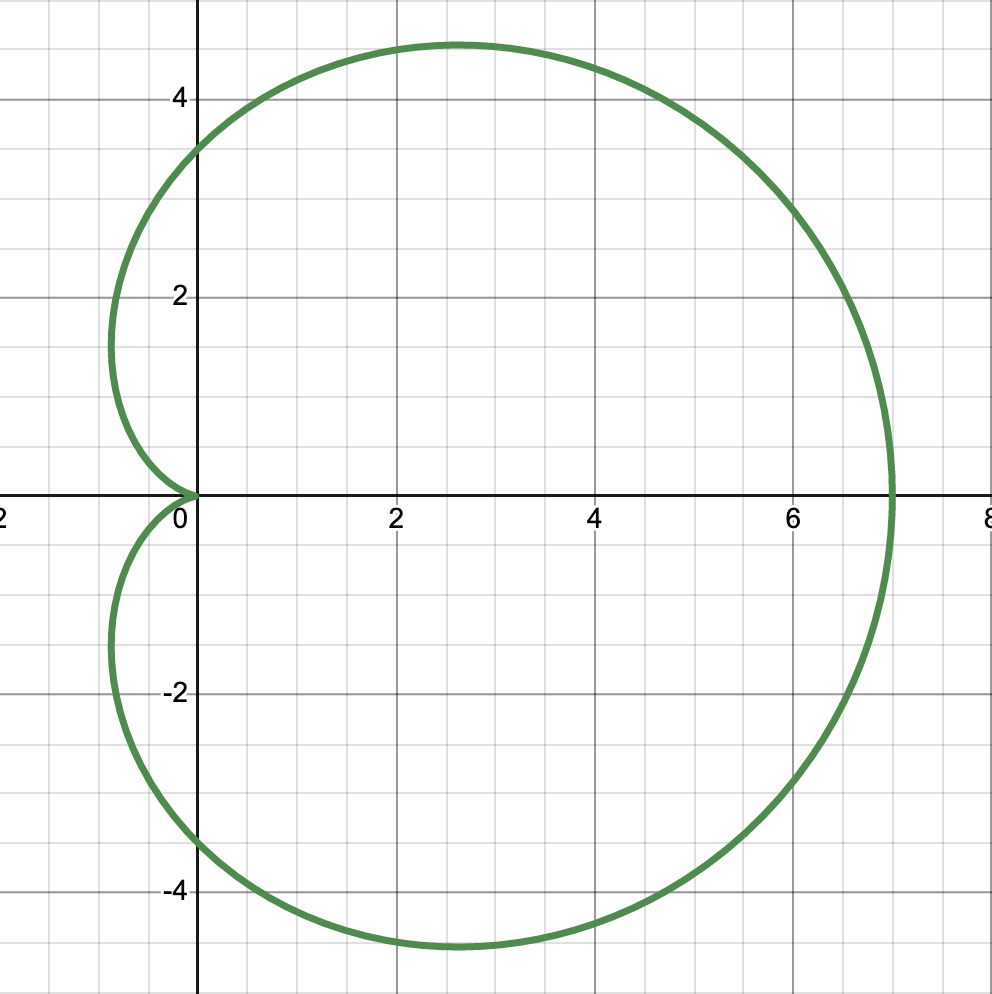
\includegraphics[width=5cm]{Pictures/Polar Form/EqualReflect.png}
        \caption[]{$a=b$ \footnotemark[2]}
        \label{a=b}
    \end{figure}
    \begin{figure}[H]
        \centering
        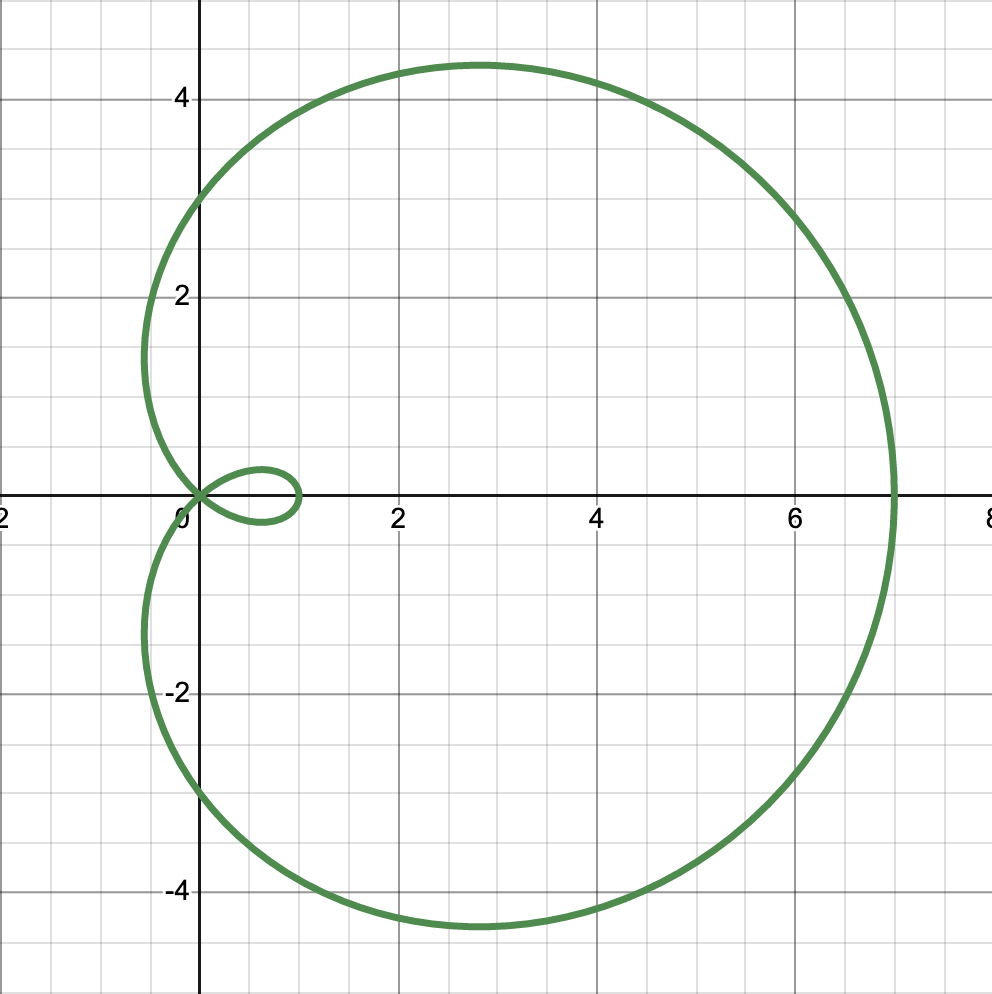
\includegraphics[width=5cm]{Pictures/Polar Form/SmallerReflect.png}
        \caption[]{$a<b$ \footnotemark[2]}
        \label{a<b}
    \end{figure}
    \end{multicols}
    
    \newpage
    
    \begin{equation}
        a-b\sin{(\theta)}
    \end{equation}
    
    \begin{multicols}{3}
    \begin{figure}[H]
        \centering
        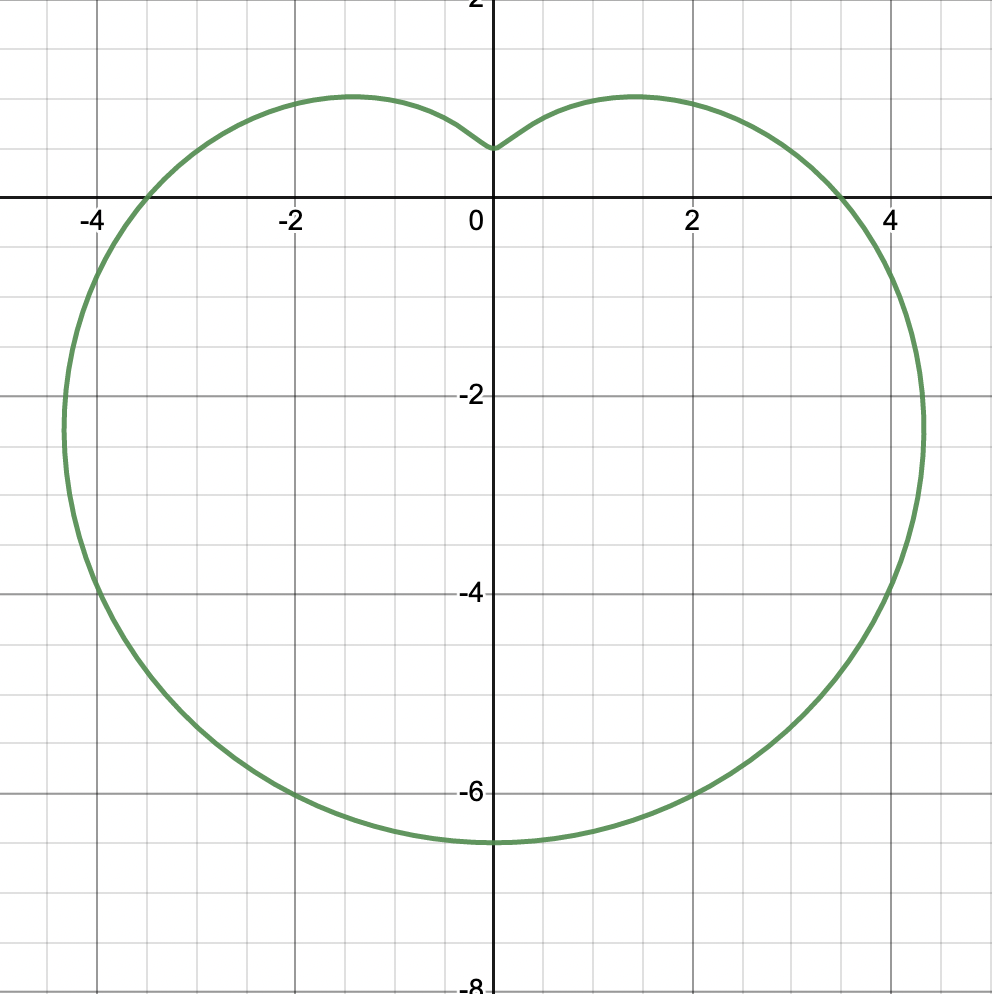
\includegraphics[width=4cm]{Pictures/Polar Form/SinBigger.png}
        \caption[]{$a>b$ \footnotemark[2]}
        \label{a>b}
    \end{figure}
    \begin{figure}[H]
        \centering
        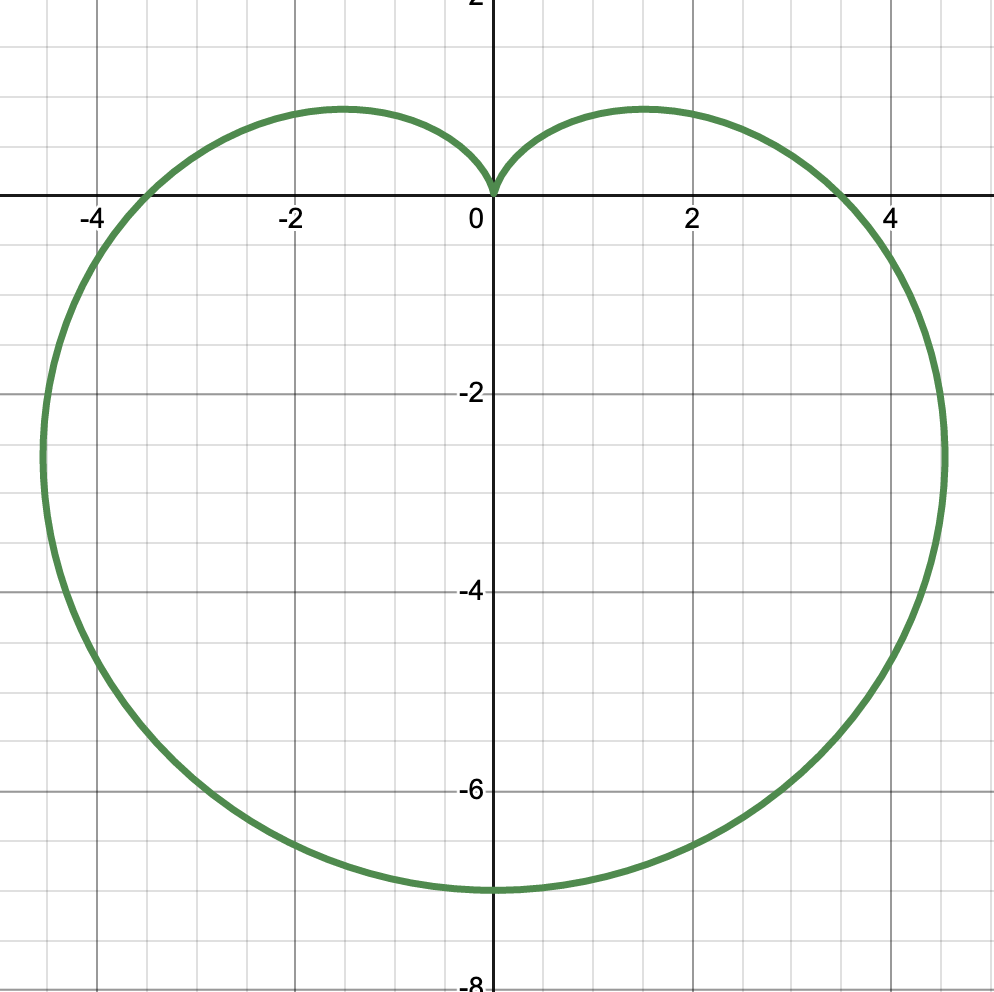
\includegraphics[width=4cm]{Pictures/Polar Form/SinEqual.png}
        \caption[]{$a=b$ \footnotemark[2]}
        \label{a=b}
    \end{figure}
    \begin{figure}[H]
        \centering
        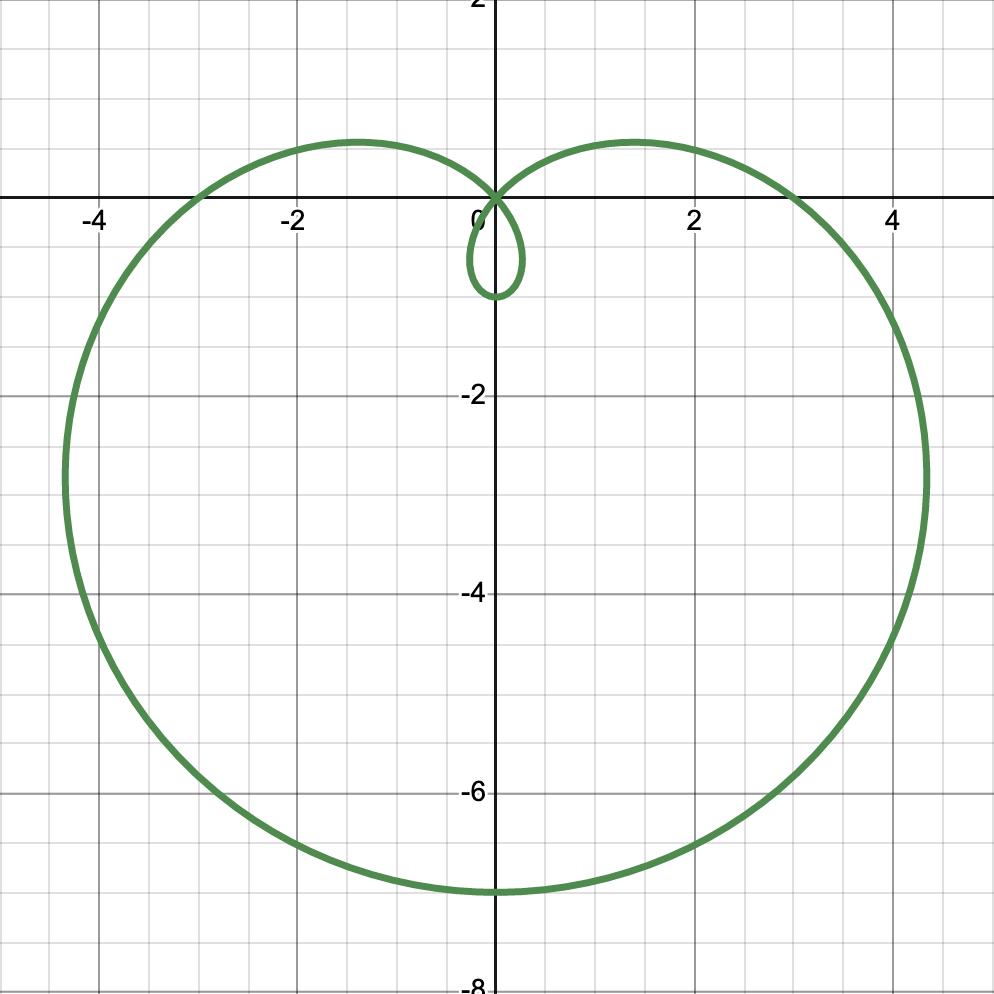
\includegraphics[width=4cm]{Pictures/Polar Form/SinSmaller.png}
        \caption[]{$a<b$ \footnotemark[2]}
        \label{a<b}
    \end{figure}
    \end{multicols}
    \footnotetext[2]{Created using Desmos}
    
    \begin{equation}
        a+b\sin{(\theta)}
    \end{equation}
    \begin{multicols}{3}
    \begin{figure}[H]
        \centering
        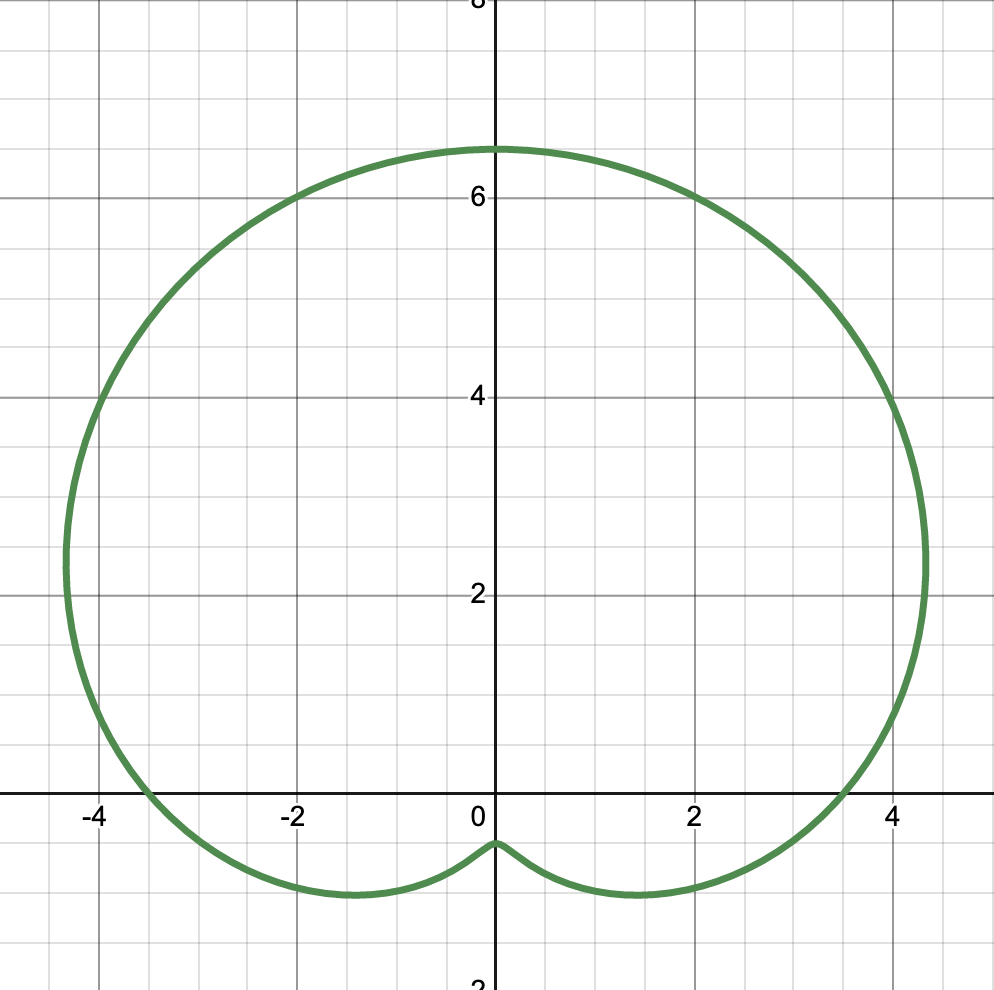
\includegraphics[width=4cm]{Pictures/Polar Form/SinBiggerReflect.png}
        \caption[]{$a>b$ \footnotemark[2]}
        \label{a>b}
    \end{figure}
    \begin{figure}[H]
        \centering
        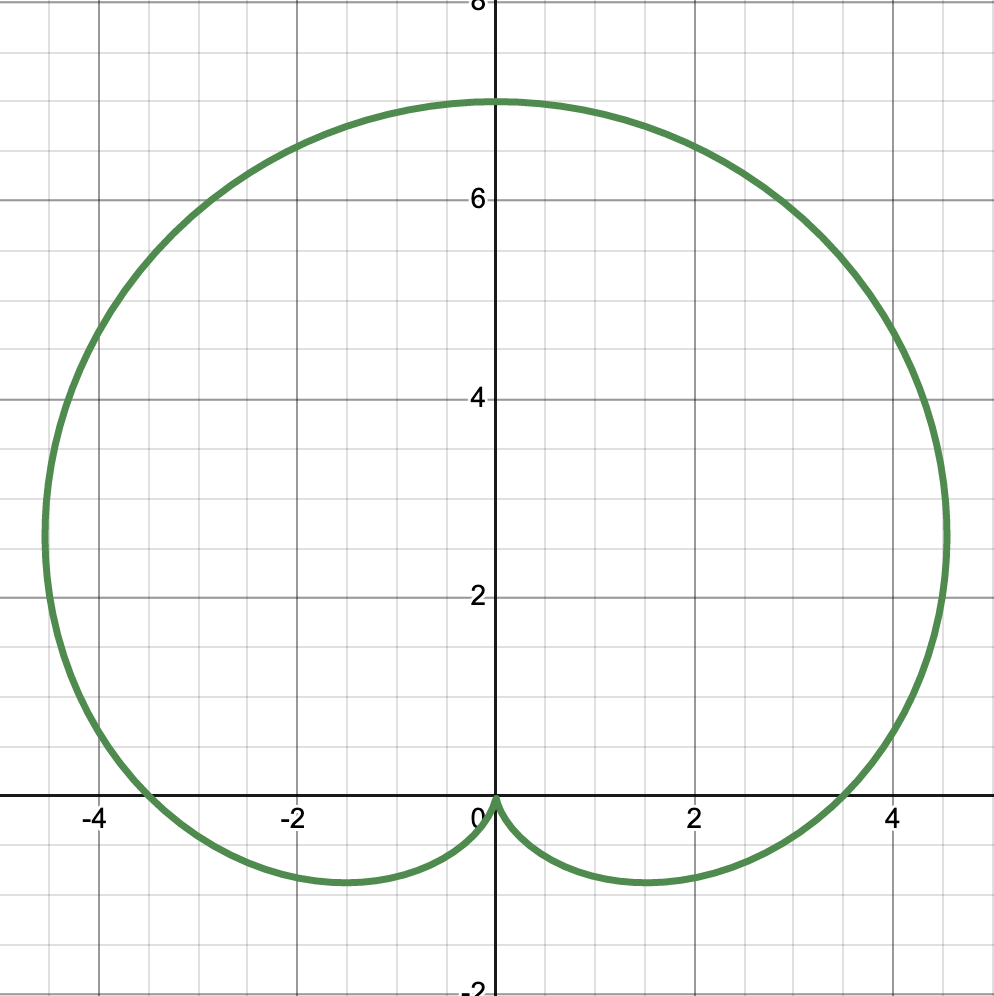
\includegraphics[width=4cm]{Pictures/Polar Form/SinEqualReflect.png}
        \caption[]{$a=b$ \footnotemark[2]}
        \label{a=b}
    \end{figure}
    \begin{figure}[H]
        \centering
        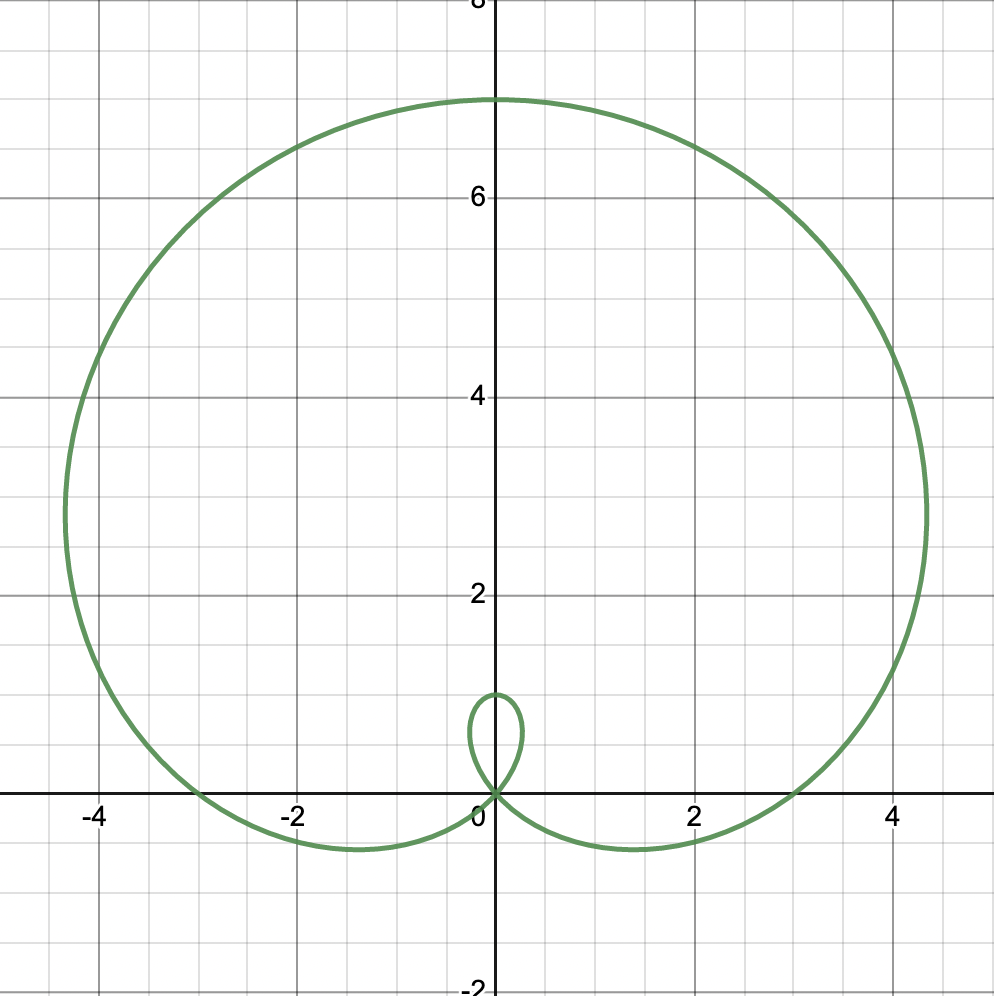
\includegraphics[width=4cm]{Pictures/Polar Form/SinSmallerReflect.png}
        \caption[]{$a<b$ \footnotemark[2]}
        \label{a<b}
    \end{figure}
    \end{multicols}

\subsection{Area of Polar Form}
\subsubsection{Area of one polar equation}
\begin{equation}
    A=\frac{1}{2}\int^b_ar^2d\theta
\end{equation}
\subsubsection{Area between two polar equations}
\begin{equation}
    A=\frac{1}{2}\int^b_ar_1^2-r_2^2d\theta
\end{equation}

\subsection{Curve Length of Polar Form}
\begin{equation}
    L=\int^b_a\sqrt{r^2+\left(\frac{dr}{d\theta}\right)^2}d\theta
\end{equation}